% !TeX program = XeLaTeX
\documentclass[11pt,letterpaper]{article}

\usepackage[utf8]{inputenc}
\usepackage[T1]{fontenc}
\usepackage[spanish,es-tabla]{babel}
\usepackage[margin=2.2cm]{geometry}
\usepackage{microtype}
\usepackage{booktabs}
\usepackage{array}
\usepackage{xcolor}
\usepackage{graphicx}
\usepackage{eso-pic}
\usepackage{titlesec}
\usepackage{caption}
\usepackage[colorlinks=true,linkcolor=black,citecolor=blue!50!black,urlcolor=blue!50!black]{hyperref}

\setlength{\parskip}{3pt}
\setlength{\parindent}{0pt}
\titlespacing*{\section}{0pt}{8pt}{2pt}
\titlespacing*{\subsection}{0pt}{5pt}{1pt}
\titleformat{\section}{\large\bfseries}{\thesection.}{0.5em}{}
\titleformat{\subsection}{\normalsize\bfseries}{\thesubsection}{0.5em}{}
\captionsetup{font=small,skip=3pt}
\setlength{\textfloatsep}{8pt}
\setlength{\intextsep}{6pt}

\newcommand{\pend}[1]{\textcolor{red}{[\textbf{COMPLETAR:} #1]}}
\newcolumntype{P}[1]{>{\raggedright\arraybackslash}p{#1}}
\newcommand{\ugm}{$\mu$g/m$^{3}$}
\newcommand{\Othree}{O$_3$}
\newcommand{\NOx}{NO$_X$}

\begin{document}

\begin{titlepage}
\AddToShipoutPictureBG*{%
  \put(-364,-565){
\includegraphics[width=707pt]{img/tec_watermark.png}}%
}
\centering
\vspace*{1.2cm}

\includegraphics[width=6.6cm]{img/tec_logo.png}

\vspace{4.2cm}
{\Large\bfseries Datos en el Aire: An\'alisis Multivariado de la Calidad del Aire en la Zona Metropolitana de Monterrey\par}
\vspace{0.3cm}
{\large Entregable 2, Etapa 2: Ruta de an\'alisis y exploraci\'on descriptiva orientada al objetivo\par}

\vspace{2.2cm}
Miembros\\
Equipo 3\\[4pt]
Ricardo Ballesteros Amavizca \hfill A01255358\\
Landon Mauricio Trevi\~no Ortiz \hfill A01199312\\
Josu\'e Olvera Zozaya \hfill A00842044\\[4pt]
Repositorio: \url{https://github.com/Ricardo-B04/sima-monitoreo-ambiental}

\vfill
Profesores: Blanca Rosa Ruiz Hern\'andez y Jes\'us Armenta Segura\\
Tecnol\'ogico de Monterrey -- Campus Monterrey\\
\today
\vspace*{1cm}
\end{titlepage}

%-------------------------------------------------------------
\section{Objetivo de indagaci\'on}
El objetivo es el mismo que en la Etapa 1; no se modific\'o. \textbf{Pregunta:} \textquestiondown c\'omo se relacionan las concentraciones de ozono con sus precursores (NO, NO$_2$, \NOx) y con las variables meteorol\'ogicas (temperatura, radiaci\'on solar, viento, humedad y presi\'on) en las estaciones de SIMA entre 2020 y 2025, y qu\'e combinaci\'on de estas variables permite explicar y clasificar los episodios de excedencia de ozono? \textbf{Objetivo general:} identificar y cuantificar, mediante t\'ecnicas de an\'alisis multivariado, la relaci\'on entre el ozono, sus precursores y la meteorolog\'ia en la ZMM para explicar y clasificar los episodios de excedencia. Se mantienen las decisiones de preparaci\'on de la Etapa 1: unidad de an\'alisis estaci\'on--d\'ia, periodo de modelado 2021--2025 (2020 s\'olo se describe por su baja cobertura) y excedencia definida como m\'aximo diario de la media m\'ovil de 8\,h por encima de 60\,ppb (criterio principal) o 51\,ppb (criterio 2026), constantes en todo el periodo \cite{sinaica}.

%-------------------------------------------------------------
\section{Ruta de an\'alisis propuesta}
La Tabla~\ref{tab:ruta} resume las t\'ecnicas previstas \cite{johnson2007}. El orden va de lo descriptivo a lo predictivo: primero se reduce y agrupa la informaci\'on sin usar la excedencia (PCA y conglomerados), luego se prueba si los grupos difieren y, al final, se modela y clasifica. Los modelos supervisados se validar\'an por bloques temporales (entrenar con 2021--2024 y evaluar en 2025) y dejando una estaci\'on fuera, porque los d\'ias consecutivos de una misma estaci\'on no son independientes.

\begin{table}[h]
\centering
\footnotesize
\renewcommand{\arraystretch}{1.05}
\begin{tabular}{@{}P{2.1cm}P{3.6cm}P{5.3cm}P{4.6cm}@{}}
\toprule
T\'ecnica & Qu\'e permitir\'a estudiar & Variables y funci\'on & Por qu\'e es adecuada \\
\midrule
Componentes principales (PCA) & Ejes que resumen la variaci\'on conjunta de precursores y meteorolog\'ia. & Interdependencia (sin variable respuesta): $\log$ NO, $\log$ NO$_2$, $\log$ \NOx{} 06--09\,h, temperatura m\'axima, radiaci\'on, humedad, viento ($u$, $v$, velocidad) y presi\'on, estandarizadas; \Othree{} y estaci\'on s\'olo para interpretar. & Las variables est\'an correlacionadas (Fig.~\ref{fig:asoc}b); el PCA elimina la redundancia y da componentes ortogonales para modelos posteriores. \\
Conglomerados (Ward y $k$-medias) & (a) Grupos de estaciones con perfil similar; (b) tipolog\'ias de d\'ias. & (a) Objeto: estaci\'on; atributos: perfil medio estandarizado. (b) Objeto: estaci\'on--d\'ia; atributos: componentes del PCA. & Formaliza el gradiente entre estaciones (Fig.~\ref{fig:est}) y permite ver si ciertos tipos de d\'ia concentran excedencias. \\
$T^2$ de Hotelling / MANOVA & Si el vector de medias difiere entre d\'ias con y sin excedencia y entre sectores. & Respuesta: vector de predictores; factores: excedencia, sector. & Prueba multivariada que precede al discriminante; controla el error tipo I frente a muchas pruebas $t$. \\
Regresi\'on lineal m\'ultiple & Cu\'anto cambia el \Othree{} con cada variable, manteniendo las dem\'as constantes. & Dependiente: \Othree{} m\'aximo de 8\,h (ppb). Independientes: precursores (\NOx{} \emph{o} NO y NO$_2$), meteorolog\'ia, ciclo anual; estaci\'on como \emph{dummies} (control). & Respuesta continua y aproximadamente sim\'etrica (asimetr\'ia 0.6); cuantifica efectos y permite separar meteorolog\'ia de tendencia entre a\~nos. \\
An\'alisis discriminante (lineal y cuadr\'atico) & Qu\'e combinaci\'on de variables separa los d\'ias con y sin excedencia. & Agrupaci\'on: excedencia (60 y 51\,ppb). Discriminantes: predictores continuos o componentes del PCA. & Es la t\'ecnica del objetivo 5; el cuadr\'atico se justifica si las covarianzas difieren entre grupos (Secc.~\ref{sec:asoc}). \\
Regresi\'on log\'istica & Probabilidad de excedencia (comparaci\'on con el discriminante). & Dependiente: excedencia; independientes: los del discriminante m\'as estaci\'on. & No exige normalidad multivariada ni covarianzas iguales; admite la estaci\'on como factor. \\
\bottomrule
\end{tabular}
\caption{Ruta de an\'alisis: t\'ecnicas, variables y funci\'on de cada una.}
\label{tab:ruta}
\end{table}

%-------------------------------------------------------------
\section{Datos y variables relevantes}
Se usa la base diaria limpia de la Etapa 1 (\texttt{sima\_diaria\_estacion.csv}): 15 estaciones $\times$ 1,826 d\'ias de 2021--2025 = 27,390 estaci\'on--d\'ias, de los cuales 24,931 (91.0\,\%) tienen ozono v\'alido y 19,585 (71.5\,\%) tienen ozono y todas las variables del modelo. Un valor diario requiere al menos 18 horas v\'alidas. La Tabla~\ref{tab:vars} describe las variables.

\begin{table}[h]
\centering
\footnotesize
\renewcommand{\arraystretch}{1.03}
\setlength{\tabcolsep}{4pt}
\begin{tabular}{@{}P{2.2cm}P{3.4cm}P{1.6cm}P{3.3cm}r P{3.1cm}@{}}
\toprule
Variable & Significado & Tipo, unidad & M\'in--m\'ax [mediana; RIC] & Falt. \% & Valores inusuales / notas \\
\midrule
Estaci\'on & Sitio de monitoreo; se agrupa en sector (poniente, centro, oriente) & Nominal, 15 niveles & -- & 0 & NO3 con 51.6\,\% de d\'ias v\'alidos de \Othree{} \\
Fecha (calendario) & Mes, temporada, fin de semana, ciclo anual & Temporal & 2021-01-01 a 2025-12-31 & 0 & -- \\
\Othree{} m\'ax. 8\,h & M\'aximo diario de la media m\'ovil de 8\,h & Continua, ppb & 2.5--123.9 [43.6; 33.8--54.6] & 9.0 & Asimetr\'ia 0.6; extremos plausibles conservados \\
Excedencia & \Othree{} m\'ax. 8\,h $>$ 60 (o 51) ppb & Binaria & 16.9\,\% (32.0\,\%) de d\'ias ``s\'i'' & 9.0 & Clases desbalanceadas \\
NO, NO$_2$ & Medias diarias de los precursores & Continua, ppb & 0.5--298 [7.2; 4.5--13.5]; 0.1--84 [12.9; 8.6--19.0] & 11.1; 10.9 & Asimetr\'ia 4.1 y 1.4: se usa $\log(1+x)$ \\
\NOx{} 06--09\,h & Media de \NOx{} de 06 a 09\,h (tr\'afico matutino) & Continua, ppb & 0.7--394 [26.7; 16.7--46.1] & 9.9 & Asimetr\'ia 2.5; \NOx{} $\neq$ NO\,+\,NO$_2$ en 1\,\% de horas \\
Temp. m\'axima & M\'aximo diario de TOUT & Continua, $^\circ$C & $-$0.6--45.1 [30.3; 25.1--33.9] & 8.9 & M\'inimo real: helada de feb.\ 2021 \\
Radiaci\'on & Media diaria de SR & Continua, kW/m$^2$ & 0--0.79 [0.15; 0.09--0.20] & 7.4 & 146 d\'ias $>$0.4 (90 en NE2--2021, 51 en NO2): posible falla de escala \\
Humedad & Media diaria de RH & Continua, \% & 1.5--96.1 [57.8; 47.5--67.3] & 13.0 & 71 d\'ias $<$10\,\%, poco plausibles \\
Viento: vel., $u$, $v$ & Velocidad media y componentes este--oeste ($u$) y norte--sur ($v$), derivadas de WSR y WDR & Continua, km/h & vel.\ 0.7--26.1 [8.1]; $u$ $-$22--19 [$-$4.1] & 7.6; 9.4 & $u<0$ en 85.5\,\% de los d\'ias: viento predominante del este \\
Presi\'on & Media diaria de PRS & Continua, mmHg & 682--748 [714.5; 710--722] & 6.5 & Depende de la altitud: se usa como anomal\'ia por estaci\'on \\
\bottomrule
\end{tabular}
\caption{Variables del an\'alisis (estaci\'on--d\'ias de 2021--2025). Falt.: porcentaje de los 27,390 estaci\'on--d\'ias sin valor diario v\'alido. RIC: rango intercuart\'ilico.}
\label{tab:vars}
\end{table}

\textbf{La estaci\'on de monitoreo.} Las 15 estaciones difieren en altitud (334 a 702\,msnm), en exposici\'on a emisiones y en su posici\'on respecto del viento dominante, por lo que una misma combinaci\'on de precursores y meteorolog\'ia no tiene por qu\'e producir el mismo ozono en todas. Se incorpora de cuatro formas: (1) como factor de comparaci\'on, individualmente y agrupada en tres sectores seg\'un la zona de SIMA (poniente: NO, NO2, NO3, SO, SO2; centro: CE, NTE, NTE2, SUR; oriente: NE, NE2, NE3, SE, SE2, SE3); (2) centrando las variables por estaci\'on (anomal\'ias), para separar la variaci\'on d\'ia a d\'ia de las diferencias fijas de ubicaci\'on, lo cual es indispensable para la presi\'on; (3) como variable \emph{dummy} de control en las regresiones; y (4) como objeto de los conglomerados y como bloque de validaci\'on.

%-------------------------------------------------------------
\section{Exploraci\'on descriptiva orientada al objetivo}

\subsection{\textquestiondown Difiere el ozono entre estaciones?}
\begin{figure}[h]
\centering
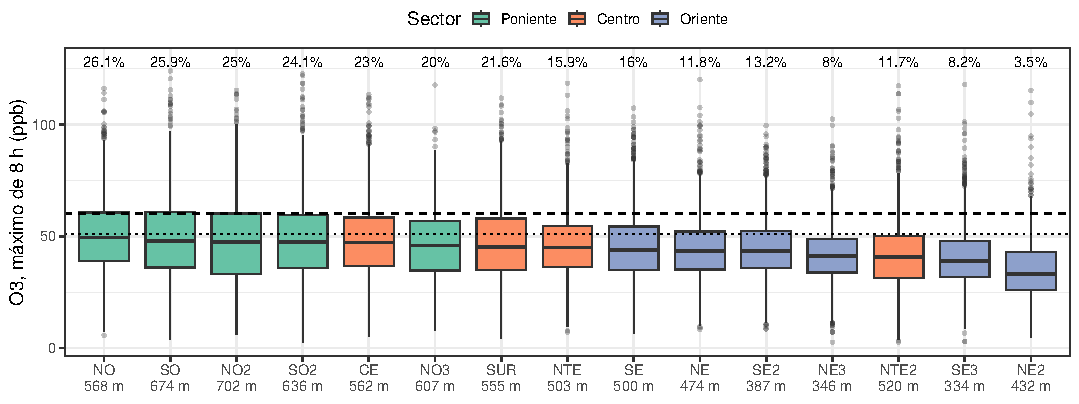
\includegraphics[width=\textwidth]{img/fig1_estaciones.pdf}
\caption{\Othree{} m\'aximo de 8\,h por estaci\'on (2021--2025), ordenadas por mediana; bajo cada estaci\'on, su altitud. Arriba, porcentaje de d\'ias $>$60\,ppb. L\'ineas: 60\,ppb (discontinua) y 51\,ppb (punteada).}
\label{fig:est}
\end{figure}

S\'i, y de forma ordenada en el espacio (Fig.~\ref{fig:est}; detalle en Anexo~\ref{tab:anexo-est}). La mediana del sector poniente es 47.8\,ppb con 24.6\,\% de d\'ias sobre 60\,ppb, frente a 44.4\,ppb y 18.1\,\% en el centro y 40.6\,ppb y 10.1\,\% en el oriente. La mediana de cada estaci\'on se asocia con su altitud ($\rho$ de Spearman = 0.87, $n=15$), pero la altitud y la longitud est\'an casi confundidas ($\rho=-0.97$): las estaciones altas son las del poniente, que quedan viento abajo del flujo predominante del este. Con estos datos no se puede separar el efecto de la altura del transporte. NE2 (Apodaca) y NTE2 (Universidad) tienen el ozono m\'as bajo de su sector y la \NOx{} mediana m\'as alta de la red (30.9 y 36.3\,ppb), compatible con consumo local de ozono por NO \cite{seinfeld2016}. Para el objetivo, la estaci\'on debe controlarse antes de atribuir efectos a la meteorolog\'ia.

\subsection{\textquestiondown C\'omo cambia en el a\~no, entre a\~nos y por tipo de d\'ia?}
\begin{figure}[h]
\centering
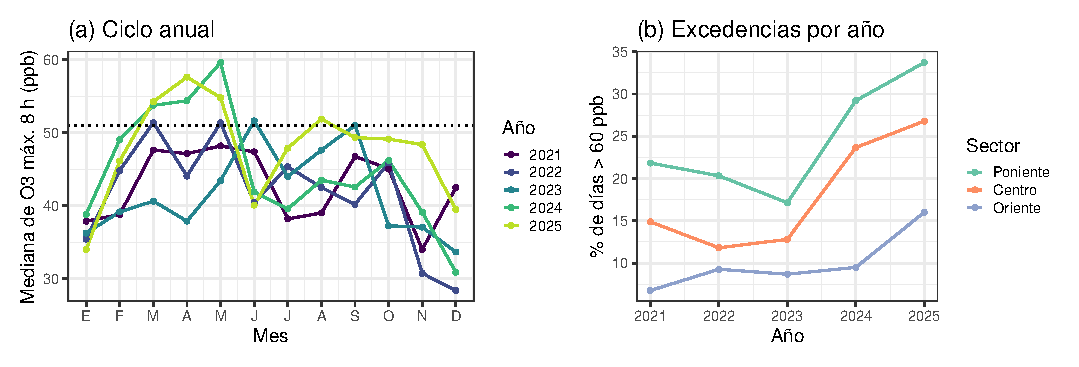
\includegraphics[width=\textwidth]{img/fig2_temporal.pdf}
\caption{(a) Mediana mensual del \Othree{} m\'aximo de 8\,h por a\~no (l\'inea punteada: 51\,ppb). (b) Porcentaje de d\'ias con excedencia ($>$60\,ppb) por a\~no y sector.}
\label{fig:temp}
\end{figure}

El ciclo anual es bimodal (Fig.~\ref{fig:temp}a; Anexo~\ref{tab:anexo-mes}): el porcentaje de excedencias sube en marzo--mayo (m\'aximo en mayo, 31.5\,\%), baja en julio (12.0\,\%) y repunta en septiembre--octubre (alrededor de 21\,\%); diciembre y enero tienen menos de 5\,\%. El descenso de verano ocurre con las temperaturas m\'aximas m\'as altas del a\~no (34--35\,$^\circ$C), pero tambi\'en con la mayor velocidad de viento y la menor \NOx{}, de modo que la temperatura por s\'i sola no explica la estacionalidad. Esto coincide con lo reportado en la ZMM, donde la meteorolog\'ia gobierna el ciclo estacional del ozono \cite{persistent2026}.

Entre a\~nos, con el umbral fijo de 60\,ppb, el porcentaje de excedencias fue 13.6, 13.2 y 12.6\,\% en 2021--2023 y subi\'o a 19.9\,\% en 2024 y 24.7\,\% en 2025 (Fig.~\ref{fig:temp}b). El aumento aparece en los tres sectores y en 13 de 15 estaciones (mediana de +6.4 puntos porcentuales), por lo que no se debe s\'olo al cambio de norma ni a qu\'e estaciones reportaron. Sin embargo, 2025 tambi\'en fue el a\~no m\'as c\'alido (mediana de temperatura m\'axima 31.0 frente a 29.9--30.3\,$^\circ$C), as\'i que falta controlar la meteorolog\'ia para saber si hay un deterioro real. Por tipo de d\'ia, en fin de semana la \NOx{} matutina baja 26\,\% (mediana de 21.6 frente a 29.2\,ppb) y el ozono no baja (44.2 frente a 43.2\,ppb), comportamiento compatible con un r\'egimen en el que reducir NO no reduce el ozono \cite{seinfeld2016}.

\subsection{\textquestiondown Qu\'e variables se asocian con el ozono y con la excedencia?}\label{sec:asoc}
\begin{figure}[h]
\centering
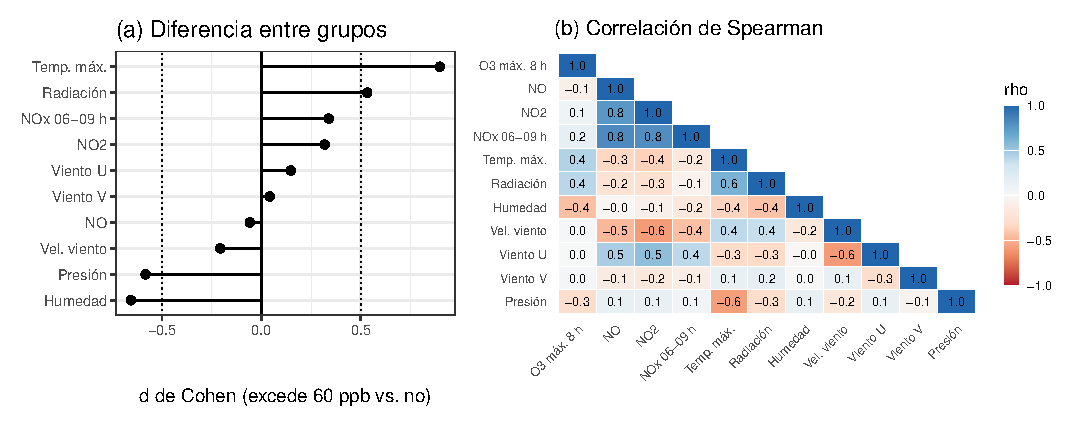
\includegraphics[width=\textwidth]{img/fig3_asociaciones.pdf}
\caption{Variables centradas por estaci\'on (2021--2025). (a) Diferencia estandarizada de medias entre d\'ias con y sin excedencia de 60\,ppb (l\'ineas punteadas: $\pm$0.5). (b) Correlaci\'on de Spearman entre \Othree{} y los predictores.}
\label{fig:asoc}
\end{figure}

Dentro de cada estaci\'on, los d\'ias con excedencia son sobre todo m\'as calurosos ($d=0.90$), m\'as secos ($d=-0.66$), de presi\'on relativamente baja ($d=-0.58$) y m\'as soleados ($d=0.53$) (Fig.~\ref{fig:asoc}a). Los precursores separan menos: NO$_2$ y \NOx{} matutina son algo mayores en los d\'ias con excedencia ($d\approx0.3$) y el NO casi no difiere. Las correlaciones con el ozono son moderadas (Fig.~\ref{fig:asoc}b): 0.44 con la temperatura, 0.41 con la radiaci\'on, $-0.45$ con la humedad, $-0.30$ con la presi\'on y $|\rho|<0.16$ con los precursores y el viento. La relaci\'on con la temperatura se mantiene en las cuatro temporadas ($\rho$ de 0.38 a 0.52). El ozono del d\'ia anterior tiene la correlaci\'on m\'as alta ($\rho=0.70$), lo que indica persistencia de los episodios. Entre predictores hay redundancia: NO, NO$_2$ y \NOx{} se correlacionan alrededor de 0.8, y la temperatura con la radiaci\'on (0.6) y con la presi\'on ($-0.6$). Adem\'as, la temperatura m\'axima var\'ia menos en los d\'ias con excedencia (raz\'on de desviaciones 0.59), se\~nal de covarianzas distintas entre grupos. Para el objetivo, esto sugiere que la meteorolog\'ia aportar\'a la mayor parte de la separaci\'on, que conviene usar componentes o una sola medida de \NOx{}, y que el discriminante cuadr\'atico o la log\'istica pueden ajustarse mejor que el lineal.

\subsection{\textquestiondown Qu\'e problemas de datos pueden influir?}
La cobertura no es homog\'enea (Anexo~\ref{fig:anexo-cob}). NO3 s\'olo tiene 468 d\'ias completos y NTE 707 (ninguno en 2025); NE tiene 6\,\% de d\'ias completos en 2025. La humedad es la variable que m\'as limita los casos completos (8.0\,\% faltante en d\'ias con ozono v\'alido). Los d\'ias excluidos por incompletos tienen algo m\'as de excedencias que los completos (18.3 frente a 16.5\,\%), un sesgo peque\~no pero en la direcci\'on de subestimar los episodios. Con la distancia de Mahalanobis, 580 casos completos (3.0\,\%) superan el percentil 99.9 de $\chi^2_{11}$; se concentran en NO2 (136) y NE2 (74), las mismas estaciones con radiaci\'on media diaria inusualmente alta, lo que apunta a un problema de sensor m\'as que a episodios reales.

%-------------------------------------------------------------
\section{S\'intesis}
\textbf{Lo descubierto.} El ozono var\'ia de forma sistem\'atica en el espacio (m\'as alto en el poniente), en el a\~no (dos m\'aximos, primavera y oto\~no) y entre a\~nos (m\'as excedencias en 2024--2025 con umbral fijo). Dentro de cada estaci\'on, la excedencia se asocia sobre todo con calor, sequedad, presi\'on baja y radiaci\'on; los precursores tienen una relaci\'on d\'ebil y no lineal con el ozono diario.

\textbf{Resultados ligados al objetivo.} El tama\~no de las diferencias entre d\'ias con y sin excedencia (Fig.~\ref{fig:asoc}a) anticipa qu\'e variables pesar\'an en el discriminante; la correlaci\'on entre predictores justifica el PCA; el gradiente entre estaciones justifica los conglomerados y el control por estaci\'on; y el aumento de 2024--2025 es la pregunta que la regresi\'on con control meteorol\'ogico debe responder.

\textbf{Limitaciones.} Cobertura desigual entre estaciones y a\~nos (NO3, NTE, NE en 2025, todo 2020); posibles fallas de sensor no detectadas por los rangos (radiaci\'on en NE2 y NO2, humedad $<$10\,\%); presi\'on dominada por la altitud; altitud y longitud confundidas; clases desbalanceadas; dependencia temporal entre d\'ias; umbrales de la NOM-020-SSA1-2021 a\'un por verificar en el Diario Oficial; y falta de compuestos org\'anicos vol\'atiles, el otro precursor del ozono.

\textbf{Lo que falta y el camino a seguir.} (1) Revisar con SIMA los valores inusuales de radiaci\'on y humedad y decidir si se invalidan; (2) PCA sobre anomal\'ias por estaci\'on; (3) conglomerados de estaciones y de d\'ias; (4) $T^2$ de Hotelling por excedencia y sector; (5) regresi\'on lineal con estaci\'on, ciclo anual y a\~no, revisando VIF y autocorrelaci\'on; (6) discriminante lineal y cuadr\'atico frente a log\'istica, con validaci\'on temporal y por estaci\'on, reportando sensibilidad y especificidad con 60 y 51\,ppb.

\textbf{Nuevas preguntas.} \textquestiondown El ozono alto del poniente se debe a la altitud o al transporte desde el oriente? \textquestiondown Por qu\'e baja en julio y agosto si son los meses m\'as calurosos? \textquestiondown El aumento de 2024--2025 persiste al controlar la meteorolog\'ia? \textquestiondown El efecto de fin de semana se repite en todas las estaciones? \textquestiondown Conviene usar el ozono del d\'ia anterior como predictor, dado que aporta mucho pero introduce dependencia temporal?

%-------------------------------------------------------------
\section{Reproducibilidad del an\'alisis}
Repositorio: \url{https://github.com/Ricardo-B04/sima-monitoreo-ambiental}. El archivo \nolinkurl{README.md} indica el orden de ejecuci\'on: \nolinkurl{analisis/01_comprension_datos.Rmd} y \nolinkurl{analisis/02_preparacion_datos.Rmd} (diagn\'ostico y limpieza; requieren los libros originales de SIMA, que no se publican) generan la base limpia \nolinkurl{datos/procesados/sima_diaria_estacion.csv}; \nolinkurl{analisis/03_exploracion_descriptiva.Rmd} parte de ese \texttt{.csv} y produce todas las cifras, tablas y figuras de este informe, y \nolinkurl{entregables/entregable2/main.tex} compila el documento.

%-------------------------------------------------------------
\section{Declaratoria de uso de inteligencia artificial}
\textbf{Opci\'on B. Se utiliz\'o IA de la siguiente forma.} \textbf{Herramienta:} Posit Assistant, asistente de IA generativa integrado en RStudio. \textbf{Uso realizado:} apoyo en el c\'odigo en R de la exploraci\'on descriptiva, el c\'alculo de cifras, las figuras y tablas y la redacci\'on de borradores. \textbf{Secciones donde se utiliz\'o:} 2 a 6 y anexos. \textbf{Validaci\'on realizada por los estudiantes:} el equipo ejecut\'o de manera independiente \nolinkurl{analisis/03_exploracion_descriptiva.Rmd} a partir de la base limpia y contrast\'o cada cifra, tabla y figura citada en el texto con la salida reproducida; adem\'as revisamos el c\'odigo generado, verificamos los supuestos estad\'isticos de cada an\'alisis y reescribimos las interpretaciones y conclusiones con criterio propio. Confirmamos que revisamos y verificamos el contenido y asumimos la responsabilidad del contenido final entregado.

%-------------------------------------------------------------
\begin{thebibliography}{9}
\small
\setlength{\itemsep}{0pt}
\bibitem{johnson2007} Johnson, R. A., \& Wichern, D. W. (2007). \textit{Applied Multivariate Statistical Analysis} (6.\textordfeminine{} ed.). Pearson Prentice Hall.
\bibitem{persistent2026} Hern\'andez-Romero, K., et al. (2026). Persistent air pollution regimes and regulatory exceedances of PM$_{10}$, PM$_{2.5}$, and O$_3$ in the Monterrey Metropolitan Area, Mexico. \textit{City and Environment Interactions}, 31, 100410. doi:10.1016/j.cacint.2026.100410
\bibitem{seinfeld2016} Seinfeld, J. H., \& Pandis, S. N. (2016). \textit{Atmospheric Chemistry and Physics: From Air Pollution to Climate Change} (3.\textordfeminine{} ed.). Wiley.
\bibitem{sinaica} SINAICA, INECC. Normas Oficiales Mexicanas de salud ambiental (NOM-020-SSA1-2021). \url{https://sinaica.inecc.gob.mx/pags/noms.php}
\end{thebibliography}

%-------------------------------------------------------------
\clearpage
\appendix
\section*{Anexos}
\renewcommand{\thetable}{A\arabic{table}}
\renewcommand{\thefigure}{A\arabic{figure}}
\setcounter{table}{0}
\setcounter{figure}{0}

\begin{table}[h]
\centering
\scriptsize
\resizebox{\textwidth}{!}{
\begin{tabular}{lllrrrrrrrrr}
\toprule
Estación & Zona & Sector & msnm & Días O3 & \% válidos & Completos & Mediana O3 & P90 O3 & \% > 60 & \% > 51 & Mediana NOx\\
\midrule
NO & Noroeste & Poniente & 568 & 1619 & 88.7 & 1189 & 49.4 & 71.7 & 26.1 & 46.3 & 18.6\\
SO & Suroeste & Poniente & 674 & 1733 & 94.9 & 1320 & 47.8 & 73.7 & 25.9 & 43.2 & 23.8\\
NO2 & Noroeste 2 & Poniente & 702 & 1765 & 96.7 & 1030 & 47.5 & 72.9 & 25.0 & 42.9 & 17.3\\
SO2 & Suroeste 2 & Poniente & 636 & 1798 & 98.5 & 1592 & 47.3 & 72.5 & 24.1 & 41.3 & 21.0\\
CE & Centro & Centro & 562 & 1712 & 93.8 & 1594 & 47.1 & 71.2 & 23.0 & 39.8 & 20.2\\
NO3 & Noroeste 3 & Poniente & 607 & 942 & 51.6 & 468 & 45.8 & 68.1 & 20.0 & 39.3 & 20.3\\
SUR & Sur & Centro & 555 & 1743 & 95.5 & 1573 & 45.2 & 70.2 & 21.6 & 37.9 & 17.3\\
NTE & Norte & Centro & 503 & 1694 & 92.8 & 707 & 44.9 & 65.0 & 15.9 & 32.9 & 17.8\\
SE & Sureste & Oriente & 500 & 1767 & 96.8 & 1556 & 43.8 & 65.8 & 16.0 & 31.4 & 17.5\\
NE & Noreste & Oriente & 474 & 1676 & 91.8 & 1162 & 43.4 & 61.4 & 11.8 & 27.8 & 19.5\\
SE2 & Sureste 2 & Oriente & 387 & 1575 & 86.3 & 1397 & 43.2 & 62.6 & 13.2 & 27.8 & 15.6\\
NE3 & Noreste 3 & Oriente & 346 & 1734 & 95.0 & 1321 & 41.0 & 58.0 & 8.0 & 20.1 & 18.9\\
NTE2 & Norte 2 & Centro & 520 & 1737 & 95.1 & 1671 & 40.6 & 61.8 & 11.7 & 23.1 & 36.3\\
SE3 & Sureste 3 & Oriente & 334 & 1769 & 96.9 & 1692 & 38.8 & 57.9 & 8.2 & 18.8 & 13.5\\
NE2 & Noreste 2 & Oriente & 432 & 1667 & 91.3 & 1313 & 33.0 & 51.1 & 3.5 & 10.1 & 30.9\\
\bottomrule
\end{tabular}
}
\caption{Resumen por estaci\'on, 2021--2025 (referido en la Secc.~4.1). Completos: d\'ias con ozono y todas las variables del modelo. \Othree{}: m\'aximo de 8\,h (ppb). \NOx{}: media diaria (ppb).}
\label{tab:anexo-est}
\end{table}

\begin{table}[h]
\centering
\small

\begin{tabular}{lrrrrrrr}
\toprule
Mes & Mediana O3 & \% > 60 & Temp. máx. & Radiación & Humedad & NOx & Viento\\
\midrule
Ene & 36.6 & 2.6 & 21.6 & 0.102 & 54 & 34.7 & 6.6\\
Feb & 44.1 & 13.6 & 24.5 & 0.136 & 52 & 31.9 & 7.3\\
Mar & 50.0 & 23.6 & 28.8 & 0.167 & 50 & 22.2 & 8.3\\
Abr & 47.0 & 22.9 & 30.6 & 0.169 & 58 & 17.4 & 9.3\\
May & 50.4 & 31.5 & 33.0 & 0.177 & 60 & 16.0 & 9.6\\
Jun & 43.8 & 20.4 & 34.5 & 0.205 & 56 & 13.9 & 10.3\\
Jul & 43.0 & 12.0 & 34.2 & 0.192 & 58 & 13.9 & 9.7\\
Ago & 45.2 & 14.4 & 35.1 & 0.192 & 54 & 14.5 & 9.4\\
Sep & 47.1 & 21.7 & 32.4 & 0.166 & 59 & 17.1 & 8.0\\
Oct & 44.2 & 21.4 & 29.0 & 0.137 & 64 & 23.8 & 7.0\\
Nov & 37.1 & 11.5 & 25.1 & 0.102 & 66 & 29.9 & 6.3\\
Dic & 34.6 & 4.8 & 23.4 & 0.091 & 63 & 41.5 & 5.7\\
\bottomrule
\end{tabular}

\caption{Medianas mensuales, 2021--2025 (referido en la Secc.~4.2). \Othree{}: m\'aximo de 8\,h (ppb); \% $>$ 60: d\'ias con excedencia; temperatura m\'axima ($^\circ$C); radiaci\'on (kW/m$^2$); humedad (\%); \NOx{} (ppb); velocidad del viento (km/h). Muestra que el descenso de julio coincide con m\'as viento y menos \NOx{}.}
\label{tab:anexo-mes}
\end{table}

\begin{figure}[h]
\centering
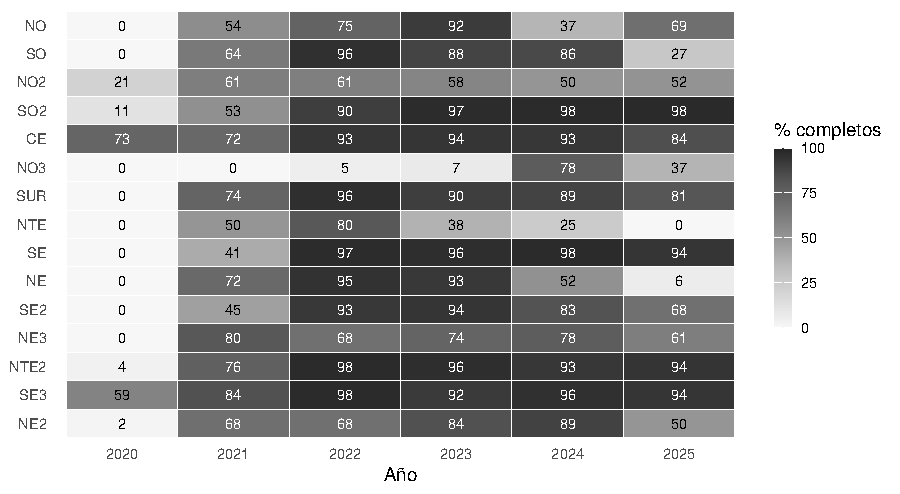
\includegraphics[width=0.8\textwidth]{img/figA1_cobertura.pdf}
\caption{Porcentaje de estaci\'on--d\'ias con ozono y todas las variables del modelo v\'alidas, por estaci\'on y a\~no (referido en la Secc.~4.4). Justifica excluir 2020 de los modelos y vigilar NO3, NTE y NE en 2024--2025.}
\label{fig:anexo-cob}
\end{figure}

\end{document}
